For a real world recognition task, an algorithm that can continuously adaptive to new labels just like the human does, is always very attractive and practical.
In this section, we propose a framework for online adaptive learning with a few labeled data in both domain and target examples using the features extracted from deep CNN.  We design the following experiment that transferring from Food-101 dataset to Food-256 dataset to illustrate our method while using just a few examples. The Food-101 and Food-256 datasets share about 46 categories of food even though the images in the same category may vary across these two datasets. The types of food in Food-101 are mainly western style while most types of food in Food-256 are typical Asian foods. To make this task more challenging, we also limited the number of examples in both source and target domain. For the rest part of this section, we first discuss the limits of some previous domain adaptation approaches for our task, then we introduce our method and show the improved performance on the same task.
\subsection{Limits of previous approaches}
From previous studies, there are two kinds of approach to solve our task. The first approach is to fine-tuning the deep CNN with the target examples incorporating with the sources ones.
Fine-tuning the deep CNN model focuses on learning good feature representations from the images and using linear models for classification. From Section \ref{sec:ft}, we successfully use this approach to transfer the knowledge from a general domain to our food domain with impressive results. Indeed, deep CNN can learn discriminative features and by taking advantage of this, this approach achieved some impressive results from previous studies\cite{Chatfield14} \cite{zeiler2014visualizing}. However, fine-tuning on deep CNN requires an ample amount of labeled target data and sometimes could degrade the performance when the labeled examples are scarce\cite{hoffman2013one}. There are many hyperparameters that affect the performance of deep CNN and fine-tuning it on a sparse label condition can lead to horrible overfitting. Apart from its sensitivity to the hyperparameters, fine-tuning the whole network requires intensive computational resources which makes it inappropriate for online learning.

Rather than learning efficient representations, another typical approach are more focused on dealing with the representation learned from conventional feature extraction methods for domain adaptation. Many methods have been proposed by minimizing the representation distance between the source and target domain in an unsupervised manner \cite{gong2012geodesic}\cite{fernando2013unsupervised}. Supervised domain adaptation models, such as Adaptive-SVM and PMT-SVM, try to utilize the knowledge from source domain and apply to target domain\cite{yang2007adapting}\cite{aytar2011tabula}. These methods are limited in our task for the following reasons: all these methods try to find the similarity between the source and target domain. Indeed, they show some good performance when these two domains have many overlapped or similar categories. From empirical experiments, we find that they suffer when the target domain is different from the source one. As far as we know, few study has shown that there is an approach that can learn new categories with a few examples.
\subsection{our method}
Chu et al. recently proposed a warm start approach for parameter selection in linear model. By iteratively updating the parameters from previous knowledge, the algorithm can search the optimal value for a specific task\cite{chuwarm}. Inspired by this, we propose a warm start adaptive learning algorithm that can adapt new categories from the target domain in an online learning scenario. Our method uses logistic regression to classify the representation obtained from deep CNN. For a new category in target domain, rather than utilizing the parameters from source domain, we introduce another affiliated binary predictor pre-trained using all the examples as the negative class and warm start the pre-trained predictor while a new category comes. This approach can be extended into an online domain adaptation scenario. Considering $M$ categories in the source domain $S$ and a new category $t$ from target domain $t$, we can train $M$ binary predictors $F=\left\{ {{f}\left( {{w_i},{b_i}} \right)} \right\}_{i = 1}^M$ for each category in $S$ and the affiliated predictor $\hat{f}=f(\hat{w},\hat{b})$ using all the examples in $\mathcal{P^-}=S$ as negative examples. The predictor $f_t$ for the new category $T$ is initialized with $\left\{\hat{w},\hat{b}\right\}$ and trained with $\mathcal{P^-}\bigcup\mathcal{P^+}$ while $\mathcal{P^+}=t$. Then we update the affiliated predictor with $\mathcal{P^-}=S\bigcup t$.
\begin{algorithm}
  \caption{Warm start online adaptation}\label{algo:ws}
  \begin{algorithmic}[1]
    \REQUIRE Source domain $S = \{ {s_i}|i = 1,..M\} $, Target domain $T = \{ {t_j}|j = 1,..N\} $, Classifier $F\leftarrow \{\emptyset\}$
    \ENSURE $F$\\
    \FORALL {$i\in M$}
         \STATE $\mathcal{P^+}\leftarrow s_i, \mathcal{P^-}\leftarrow S-s_i$\\
          Train ${{f_i}\left( {{w_i},{b_i}} \right)}$ with $\mathcal{P^+}\bigcup\mathcal{P^-}$, $F\leftarrow F\bigcup f_i$        
    \ENDFOR
    \STATE Training affiliated $\hat{f}\left( {{w_i},{b_i}} \right)$ with $\mathcal{P^-}=S$
    \WHILE {$t_j  \notin S$}
         \FORALL {$i\in M$}
             \STATE $\mathcal{P^+}\leftarrow s_i, \mathcal{P^-}\leftarrow S-s_i+t_j$ \\
              Update ${{f_i}\left( {{w_i},{b_i}} \right)}$ with $\mathcal{P^+}\bigcup\mathcal{P^-}$
        \ENDFOR
        \STATE Initialize $\hat{f_j}$ with $\left\{\hat{w},\hat{b}\right\}$ and train.
        \STATE $F\leftarrow\ F\bigcup \hat{f_j}$ 
        \STATE $D\leftarrow D\bigcup t_j, M\leftarrow M+1$ 
     \ENDWHILE
  \end{algorithmic}
\end{algorithm} 

\begin{figure*}
  \centering
  % Requires \usepackage{graphicx}
  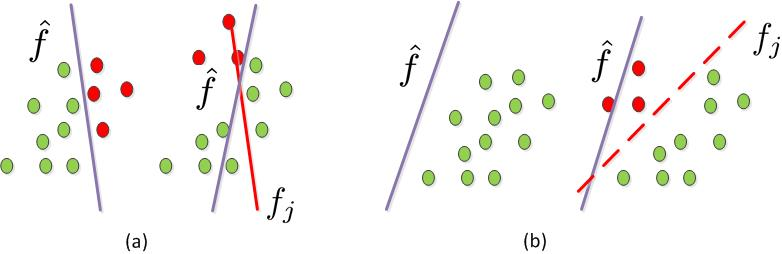
\includegraphics[scale = .6]{fig/domain.jpg}\\
  \caption{ASVM vs Ap}
\end{figure*}
